%----------------------------------------------------------------------------------------
%	PACKAGES AND OTHER DOCUMENT CONFIGURATIONS
%----------------------------------------------------------------------------------------

% Pakcages
\documentclass[12pt,a4paper]{report}
\usepackage[english]{babel}
\usepackage[utf8x]{inputenc}
\usepackage{amsmath}
\usepackage{graphicx}
\usepackage{float}
\usepackage[colorinlistoftodos]{todonotes}
\usepackage{listings}
\usepackage{xcolor}
\usepackage{tikz} \usetikzlibrary{shapes,arrows,positioning, arrows.meta}
\usepackage{fancyhdr}
\usepackage{titlesec}
\usepackage{tocloft}
\usepackage{subcaption}
\usepackage{setspace}
\usepackage[a4paper,top=3cm,bottom=2cm,left=3cm,right=3cm,marginparwidth=1.75cm]{geometry}
\usepackage{multirow}
\usepackage{tabularx}
\usepackage{booktabs}
\usepackage{threeparttable}

% Define custom colors
\definecolor{ghbggray}{HTML}{F6F8FA}
\definecolor{ghblue}{HTML}{0366D6}
\definecolor{ghgreen}{HTML}{22863A}
\definecolor{ghred}{HTML}{B31D28}
\definecolor{ghdarkgray}{HTML}{24292E}
\definecolor{ghorange}{HTML}{D73A49}

% Define code listing settings
\lstset{
    backgroundcolor=\color{ghbggray},
    commentstyle=\color{ghgreen},
    keywordstyle=\color{ghblue},
    numberstyle=\tiny\color{ghdarkgray},
    stringstyle=\color{ghred},
    basicstyle=\ttfamily\footnotesize\color{ghdarkgray},
    breakatwhitespace=false,
    breaklines=true,
    captionpos=b,
    keepspaces=true,
    numbers=left,
    numbersep=5pt,
    showspaces=false,
    showstringspaces=false,
    showtabs=false,
    tabsize=2,
    identifierstyle=\color{ghorange}
}

% Define custom page style
\renewcommand{\thesection}{\arabic{section}}
\renewcommand{\cftsecfont}{\bfseries}
\titleformat{\section}[block]{\normalfont\Large\bfseries}{\thesection}{1em}{}
\setlength{\parindent}{0pt}

% Define line spacing
\setstretch{1}

%----------------------------------------------------------------------------------------
%	COVER
%----------------------------------------------------------------------------------------

\begin{document}

\begin{titlepage}

    \newcommand{\HRule}{\rule{\linewidth}{0.5mm}}

    \center
    \vspace*{1.5cm}

    %----------------------------------------------------------------------------------------
    %	HEADING SECTIONS
    %----------------------------------------------------------------------------------------

    \includegraphics[scale=.2]{src/cuhk.png}\\[1cm]
    \textsc{\large The Chinese University of Hong Kong, Shenzhen}\\[1.5cm]

    %course code
    \textsc{\Large Course Code}\\[0.5cm]

    %course name
    \textsc{\large Course Name}\\[0.5cm]

    %----------------------------------------------------------------------------------------
    %	TITLE SECTION
    %----------------------------------------------------------------------------------------

    \HRule \\[0.4cm]
    { \huge \bfseries Your Title}
    \HRule \\[1.5cm]

    %----------------------------------------------------------------------------------------
    %	AUTHOR SECTION
    %----------------------------------------------------------------------------------------

    \begin{minipage}{0.4\textwidth}
        \begin{tabular}{l l}
            \emph{Author:\quad}     & Your Name       \\
            \emph{Student ID:\quad} & Your Student ID \\
        \end{tabular}

    \end{minipage}\\[2cm]

    %----------------------------------------------------------------------------------------
    %	DATE SECTION
    %----------------------------------------------------------------------------------------

    % Date
    {\large \today}\\[2cm]
    \vfill
\end{titlepage}

%----------------------------------------------------------------------------------------
%	CONTENTS
%----------------------------------------------------------------------------------------

\tableofcontents
\newpage

%----------------------------------------------------------------------------------------
%	HEADER AND FOOTER
%----------------------------------------------------------------------------------------

\fancypagestyle{mypagestyle}{
    \fancyhf{}
    \fancyhead[L]{\small Your Title}
    \fancyhead[R]{\small Your Student ID}
    \fancyfoot[C]{\thepage} % Add this line to include page numbers at the center of the footer
    \renewcommand{\headrulewidth}{1pt}
}

% Apply custom page style
\pagestyle{mypagestyle}

%----------------------------------------------------------------------------------------
%	MAIN BODY
%----------------------------------------------------------------------------------------

\section{Part 1}

This is an example code listing:

% Code listing
\begin{lstlisting}[language=Python, caption=Example Python code]
print("Hello World!")
\end{lstlisting}

\subsection{Subsection 1}
This is a subsection.

% Figure
\begin{figure}[h]
    \centering
    \includegraphics[width=0.3\textwidth]{src/example.png}
    \caption{Example image}
\end{figure}

\subsection{Subsection 2}
%Subfigure
\begin{figure}[h]
    \centering

    \begin{subfigure}{0.4\textwidth}
        \centering
        \includegraphics[width=\textwidth]{src/example.png}
        \caption{Caption for Image 1}
    \end{subfigure}
    \hfill
    \begin{subfigure}{0.4\textwidth}
        \centering
        \includegraphics[width=\textwidth]{src/example.png}
        \caption{Caption for Image 2}
    \end{subfigure}

    \vspace{0.5cm} % adjust vertical space between rows

    \begin{subfigure}{0.4\textwidth}
        \centering
        \includegraphics[width=\textwidth]{src/example.png}
        \caption{Caption for Image 3}
    \end{subfigure}
    \hfill
    \begin{subfigure}{0.4\textwidth}
        \centering
        \includegraphics[width=\textwidth]{src/example.png}
        \caption{Caption for Image 4}
    \end{subfigure}

    \caption{Example of the 2x2 Image Grid}
\end{figure}

\section{Part 2}
This is an example of an inline equation: $f(x)=x^2$.

This is an example of a displayed equation:

\begin{align}
    f_1(x)   & = x^2            \\
    f_2(x,y) & = f_1^2(x) + y^3
\end{align}

The sum of $A$ and $B$ is:

\[
    A + B = \begin{bmatrix}
        1+9 & 2+8 & 3+7 \\
        4+6 & 5+5 & 6+4 \\
        7+3 & 8+2 & 9+1
    \end{bmatrix}
    = \begin{bmatrix}
        10 & 10 & 10 \\
        10 & 10 & 10 \\
        10 & 10 & 10
    \end{bmatrix}
\]

% Graph
This is an example graph:
\begin{center}
    \begin{tikzpicture}[scale=0.7]
        \draw[->] (0,0) -- (5,0) node[right] {$x$};
        \draw[->] (0,0) -- (0,5) node[above] {$y$};
        \draw[scale=0.5,domain=0:4,smooth,variable=\x,blue] plot ({\x},{\x*\x});
        \node[below] at (2, -1) {$y = x^2$};
    \end{tikzpicture}
\end{center}

\section{Part 3}
% Table
\begin{table}[h]
    \centering
    \begin{tabular}{|c|c|c|}
        \hline
        \textbf{Column 1} & \textbf{Column 2} & \textbf{Column 3} \\
        \hline
        Row 1, Column 1   & Row 1, Column 2   & Row 1, Column 3   \\
        \hline
        Row 2, Column 1   & Row 2, Column 2   & Row 2, Column 3   \\
        \hline
        Row 3, Column 1   & Row 3, Column 2   & Row 3, Column 3   \\
        \hline
    \end{tabular}
    \caption{Example table}
\end{table}

\subsection{Program Framework}
This is an example graph of program framework:
\begin{center}
    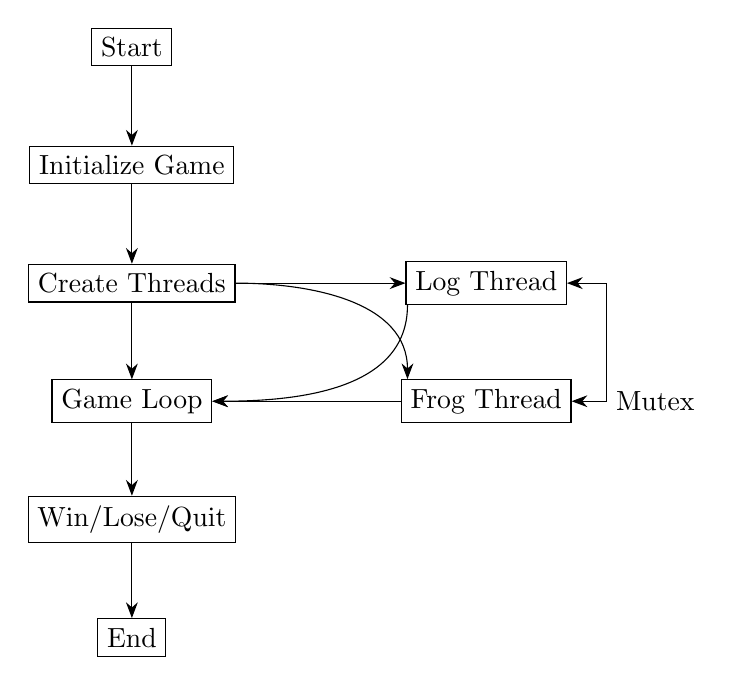
\begin{tikzpicture}[node distance=1.5cm, >={Stealth[length=2mm]}][h]

        \node (start) [draw, rectangle] {Start};
        \node (init) [draw, rectangle, below of=start] {Initialize Game};
        \node (create) [draw, rectangle, below of=init] {Create Threads};
        \node (game) [draw, rectangle, below of=create] {Game Loop};
        \node (win) [draw, rectangle, below of=game] {Win/Lose/Quit};
        \node (end) [draw, rectangle, below of=win] {End};

        \node (log) [draw, rectangle, right of=create, xshift=3cm] {Log Thread};
        \node (frog) [draw, rectangle, below of=log] {Frog Thread};

        \draw [->] (start) -- (init);
        \draw [->] (init) -- (create);
        \draw [->] (create) -- (game);
        \draw [->] (game) -- (win);
        \draw [->] (win) -- (end);

        \draw [->] (create.east) to [out=0, in=180](log.west);
        \draw [->] (create.east) to [out=0, in=90] ([xshift=-1cm] frog.north);

        \draw [->] ([xshift=-1cm] log.south) to [out=270, in=0] (game.east);
        \draw [->] (frog) to [out=180, in=0] (game.east);

        \draw [<->] (log.east) -- ++(0.5,0) |- (frog.east) node[midway,right] {Mutex};
    \end{tikzpicture}
    \captionof{figure}{Program Framework}
\end{center}

\subsection{Part 4: Table}

\renewcommand{\arraystretch}{0.85}
\begin{table}[h]
    \caption{USA}

    \centering
    \footnotesize
    \begin{tabular}{ccccccccccc}
        \toprule
                                          &                 & \multicolumn{3}{c}{1.5 hour} & \multicolumn{3}{c}{3 hour} & \multicolumn{3}{c}{6 hour}                                                                                                                                      \\
                                          & Method          & \textit{MAE}                 & \textit{RMSE}              & \multicolumn{1}{c|}{\textit{MAPE} } & \textit{MAE}   & \textit{RMSE}  & \multicolumn{1}{c|}{\textit{MAPE}}  & \textit{MAE}   & \textit{RMSE}   & \textit{MAPE}  \\ \midrule
        \multirow{11}{*}{Arrival Delay}   & HA              & 9.09                         & 11.85                      & \multicolumn{1}{c|}{1.15}           & 9.09           & 11.85          & \multicolumn{1}{c|}{1.15}           & 9.09           & 11.85           & 1.15           \\
                                          & VAR             & 7.80                         & 10.47                      & \multicolumn{1}{c|}{1.21}           & 8.12           & 10.82          & \multicolumn{1}{c|}{1.22}           & 8.48           & 11.24           & 1.22           \\
                                          & ARIMA           & 10.51                        & 13.89                      & \multicolumn{1}{c|}{2.44}           & 10.48          & 13.86          & \multicolumn{1}{c|}{2.42}           & 10.60          & 14.02           & 2.48           \\
                                          & SVM             & 8.18                         & 10.95                      & \multicolumn{1}{c|}{1.21}           & 8.49           & 11.27          & \multicolumn{1}{c|}{1.22}           & 8.74           & 11.56           & 1.21           \\
                                          & STGCN           &                              &                            & \multicolumn{1}{c|}{}               &                &                & \multicolumn{1}{c|}{}               &                &                 &                \\
                                          & Gwave           &                              &                            & \multicolumn{1}{c|}{}               &                &                & \multicolumn{1}{c|}{}               &                &                 &                \\
                                          & GAT             & 7.595                        & 10.222                     & \multicolumn{1}{c|}{1.181}          & 7.856          & 10.492         & \multicolumn{1}{c|}{1.148}          & 8.337          & 10.995          & 1.075          \\
                                          & GRU             & 7.243                        & 9.981                      & \multicolumn{1}{c|}{1.181}          & 7.466          & 10.231         & \multicolumn{1}{c|}{1.195}          & 7.761          & 10.527          & 1.164          \\
                                          & ASTGCN          & 7.312                        & 10.019                     & \multicolumn{1}{c|}{1.2}            & 7.545          & 10.277         & \multicolumn{1}{c|}{1.192}          & 8.018          & 10.714          & 1.123          \\
                                          & STPN            & 6.875                        & 9.411                      & \multicolumn{1}{c|}{0.996}          & 7.171          & 9.762          & \multicolumn{1}{c|}{1.005}          & 7.552          & 10.189          & 1.065          \\
                                          & \textbf{STCGAT} & \textbf{6.615}               & \textbf{9.221}             & \multicolumn{1}{c|}{\textbf{1.099}} & \textbf{6.947} & \textbf{9.642} & \multicolumn{1}{c|}{\textbf{1.130}} & \textbf{7.278} & \textbf{10.008} & \textbf{1.127} \\\midrule
        \multirow{11}{*}{Departure Delay} & HA              & 6.52                         & 8.63                       & \multicolumn{1}{c|}{1.28}           & 6.52           & 8.63           & \multicolumn{1}{c|}{1.28}           & 6.52           & 8.63            & 1.28           \\
                                          & VAR             & 5.56                         & 7.66                       & \multicolumn{1}{c|}{1.13}           & 5.82           & 7.93           & \multicolumn{1}{c|}{1.14}           & 6.17           & 8.30            & 1.13           \\
                                          & ARIMA           & 7.61                         & 10.55                      & \multicolumn{1}{c|}{1.13}           & 7.59           & 10.55          & \multicolumn{1}{c|}{1.12}           & 7.65           & 10.64           & 1.14           \\
                                          & SVM             & 5.96                         & 8.13                       & \multicolumn{1}{c|}{1.09}           & 6.24           & 8.41           & \multicolumn{1}{c|}{1.08}           & 6.43           & 8.65            & 1.04           \\
                                          & STGCN           &                              &                            & \multicolumn{1}{c|}{}               &                &                & \multicolumn{1}{c|}{}               &                &                 &                \\
                                          & Gwave           &                              &                            & \multicolumn{1}{c|}{}               &                &                & \multicolumn{1}{c|}{}               &                &                 &                \\
                                          & GAT             & 4.854                        & 6.989                      & \multicolumn{1}{c|}{0.964}          & 5.05           & 7.121          & \multicolumn{1}{c|}{0.942}          & 5.362          & 7.373           & 0.898          \\
                                          & GRU             & 4.569                        & 6.897                      & \multicolumn{1}{c|}{0.966}          & 4.694          & 7.019          & \multicolumn{1}{c|}{0.982}          & 4.933          & 7.201           & 0.976          \\
                                          & ASTGCN          & 4.548                        & 6.942                      & \multicolumn{1}{c|}{0.98}           & 4.693          & 7.045          & \multicolumn{1}{c|}{0.961}          & 5.115          & 7.274           & 0.965          \\
                                          & STPN            & 4.812                        & 6.787                      & \multicolumn{1}{c|}{1.063}          & 4.930          & 6.883          & \multicolumn{1}{c|}{1.073}          & 5.117          & 7.108           & 1.076          \\
                                          & \textbf{STCGAT} & \textbf{4.474}               & \textbf{6.838}             & \multicolumn{1}{c|}{\textbf{0.944}} & \textbf{4.596} & \textbf{6.912} & \multicolumn{1}{c|}{\textbf{0.948}} & \textbf{4.717} & \textbf{7.020}  & \textbf{0.950} \\\bottomrule
    \end{tabular}
\end{table}

\begin{table}[h!]
    \caption{Results on the U.S. delay dataset}
    \label{tab: US results}
    \centering
    \footnotesize
    \resizebox{0.9\linewidth}{!}{
        \tiny
        \begin{tabular}{cccccccc}
            \toprule
                                              &                 & \multicolumn{2}{c}{1.5 hour} & \multicolumn{2}{c}{3 hour} & \multicolumn{2}{c}{6 hour}                                                \\
            \cmidrule(r){3-4} \cmidrule(r){5-6} \cmidrule(r){7-8}
                                              & Method          & \textit{MAE}                 & \textit{RMSE}              & \textit{MAE}               & \textit{RMSE} & \textit{MAE} & \textit{RMSE} \\
            \midrule
            \multirow{11}{*}{Arrival Delay}   & HA              & 9.09                         & 11.85                      & 9.09                       & 11.85         & 9.09         & 11.85         \\
                                              & VAR             & 7.80                         & 10.47                      & 8.12                       & 10.82         & 8.48         & 11.24         \\
                                              & ARIMA           & 10.51                        & 13.89                      & 10.48                      & 13.86         & 10.60        & 14.02         \\
                                              & SVR             & 8.18                         & 10.95                      & 8.49                       & 11.27         & 8.74         & 11.56         \\
                                              & STGCN           &                              &                            &                            &               &              &               \\
                                              & Gwave           &                              &                            &                            &               &              &               \\
                                              & GAT             & 7.595                        & 10.222                     & 7.856                      & 10.492        & 8.337        & 10.995        \\
                                              & GRU             & 7.243                        & 9.981                      & 7.466                      & 10.231        & 7.761        & 10.527        \\
                                              & ASTGCN          & 7.312                        &                            &                            &               &              &               \\
                                              & STPN            & 6.875                        &                            &                            &               &              &               \\
                                              & \textbf{STCGAT} & \textbf{6.615}               &                            &                            &               &              &               \\ \midrule
            \multirow{11}{*}{Departure Delay} & HA              &                              &                            &                            &               &              &               \\
                                              & VAR             &                              &                            &                            &               &              &               \\
                                              & ARIMA           &                              &                            &                            &               &              &               \\
                                              & SVR             &                              &                            &                            &               &              &               \\
                                              & STGCN           &                              &                            &                            &               &              &               \\
                                              & Gwave           &                              &                            &                            &               &              &               \\
                                              & GAT             &                              &                            &                            &               &              &               \\
                                              & GRU             &                              &                            &                            &               &              &               \\
                                              & ASTGCN          &                              &                            &                            &               &              &               \\
                                              & STPN            &                              &                            &                            &               &              &               \\
                                              & \textbf{STCGAT} &                              &                            &                            &               &              &               \\ \bottomrule
        \end{tabular}
    }
\end{table}

\renewcommand{\arraystretch}{0.85}
\begin{table}[h]
    \caption{USA}
    \centering
    \footnotesize
    \begin{tabular}{ccccccccccc}
        \toprule
                                          &                 & \multicolumn{3}{c}{1.5 hour} & \multicolumn{3}{c}{3 hour} & \multicolumn{3}{c}{6 hour}                                                                                                                             \\
                                          & Method          & \textit{MAE}                 & \textit{RMSE}              & \multicolumn{1}{c|}{\textit{MAPE} } & \textit{MAE} & \textit{RMSE} & \multicolumn{1}{c|}{\textit{MAPE}} & \textit{MAE} & \textit{RMSE} & \textit{MAPE} \\ \midrule
        \multirow{11}{*}{Arrival Delay}   & HA              &                              &                            & \multicolumn{1}{c|}{}               &              &               & \multicolumn{1}{c|}{}              &              &               &               \\
                                          & VAR             &                              &                            & \multicolumn{1}{c|}{}               &              &               & \multicolumn{1}{c|}{}              &              &               &               \\
                                          & ARIMA           &                              &                            & \multicolumn{1}{c|}{}               &              &               & \multicolumn{1}{c|}{}              &              &               &               \\
                                          & SVM             &                              &                            & \multicolumn{1}{c|}{}               &              &               & \multicolumn{1}{c|}{}              &              &               &               \\
                                          & STGCN           &                              &                            & \multicolumn{1}{c|}{}               &              &               & \multicolumn{1}{c|}{}              &              &               &               \\
                                          & Gwave           &                              &                            & \multicolumn{1}{c|}{}               &              &               & \multicolumn{1}{c|}{}              &              &               &               \\
                                          & GAT             &                              &                            & \multicolumn{1}{c|}{}               &              &               & \multicolumn{1}{c|}{}              &              &               &               \\
                                          & GRU             &                              &                            & \multicolumn{1}{c|}{}               &              &               & \multicolumn{1}{c|}{}              &              &               &               \\
                                          & ASTGCN          &                              &                            & \multicolumn{1}{c|}{}               &              &               & \multicolumn{1}{c|}{}              &              &               &               \\
                                          & STPN            &                              &                            & \multicolumn{1}{c|}{}               &              &               & \multicolumn{1}{c|}{}              &              &               &               \\
                                          & \textbf{STCGAT} &                              &                            & \multicolumn{1}{c|}{}               &              &               & \multicolumn{1}{c|}{}              &              &               &               \\ \midrule
        \multirow{11}{*}{Departure Delay} & HA              &                              &                            & \multicolumn{1}{c|}{}               &              &               & \multicolumn{1}{c|}{}              &              &               &               \\
                                          & VAR             &                              &                            & \multicolumn{1}{c|}{}               &              &               & \multicolumn{1}{c|}{}              &              &               &               \\
                                          & ARIMA           &                              &                            & \multicolumn{1}{c|}{}               &              &               & \multicolumn{1}{c|}{}              &              &               &               \\
                                          & SVM             &                              &                            & \multicolumn{1}{c|}{}               &              &               & \multicolumn{1}{c|}{}              &              &               &               \\
                                          & STGCN           &                              &                            & \multicolumn{1}{c|}{}               &              &               & \multicolumn{1}{c|}{}              &              &               &               \\
                                          & Gwave           &                              &                            & \multicolumn{1}{c|}{}               &              &               & \multicolumn{1}{c|}{}              &              &               &               \\
                                          & GAT             &                              &                            & \multicolumn{1}{c|}{}               &              &               & \multicolumn{1}{c|}{}              &              &               &               \\
                                          & GRU             &                              &                            & \multicolumn{1}{c|}{}               &              &               & \multicolumn{1}{c|}{}              &              &               &               \\
                                          & ASTGCN          &                              &                            & \multicolumn{1}{c|}{}               &              &               & \multicolumn{1}{c|}{}              &              &               &               \\
                                          & STPN            &                              &                            & \multicolumn{1}{c|}{}               &              &               & \multicolumn{1}{c|}{}              &              &               &               \\
                                          & \textbf{STCGAT} &                              &                            & \multicolumn{1}{c|}{}               &              &               & \multicolumn{1}{c|}{}              &              &               &               \\ \bottomrule
    \end{tabular}
\end{table}

\begin{table}[!htbp]
    \footnotesize
    \begin{center}
        \caption{Identification of performance indicators in 33 matches}
        \begin{threeparttable}
            \begin{tabularx}{40em}{p{1em}|*{2}{>{\centering\arraybackslash}X}|*{2}{>{\centering\arraybackslash}X}|*{2}{>{\centering\arraybackslash}X}|*{2}{>{\centering\arraybackslash}X}|*{2}{>{\centering\arraybackslash}X}|p{2em}}
                \toprule
                \multirow{2}{*}{ID} & \multicolumn{2}{c|}{Coordination} & \multicolumn{2}{c|}{Distribution} & \multicolumn{2}{c|}{Tempo} & \multicolumn{2}{c|}{Flexibilty} & \multicolumn{2}{c|}{Pressing} & \multirow{2}{*}{\small Result}                                                                       \\
                \cmidrule{2-11}
                                    & H\tnote{***}                      & O                                 & H                          & O                               & H                             & O                              & H     & O     & H     & O     &                                     \\
                \midrule
                1                   & 7.61                              & 4.00                              & 62.25                      & 12.60                           & 539.50                        & \small 1476.57                 & 32.42 & 28.58 & 42.37 & 51.23 & \multicolumn{1}{c}{\centering win}  \\
                2                   & 2.88                              & 8.25                              & 28.71                      & 11.17                           & \small 1019.95                & 692.49                         & 29.30 & 27.34 & 46.36 & 49.81 & \multicolumn{1}{c}{\centering tie}  \\
                3                   & 5.10                              & 9.00                              & 8.43                       & 34.17                           & 634.78                        & 596.98                         & 27.77 & 27.03 & 40.43 & 52.02 & \multicolumn{1}{c}{\centering loss} \\
                4                   & 6.01                              & 5.66                              & 6.14                       & 62.40                           & 760.01                        & 934.64                         & 32.74 & 31.94 & 44.14 & 51.62 & \multicolumn{1}{c}{\centering loss} \\
                30                  & 5.61                              & 3.00                              & 62.25                      & 7.13                            & 707.96                        & \small 2018.52                 & 30.94 & 30.18 & 50.75 & 58.75 & \multicolumn{1}{c}{\centering win}  \\
                31                  & \textit{6.58}                     & 4.21                              & 20.10                      & 13.87                           & 986.98                        & \small 1014.37                 & 32.53 & 26.66 & 44.20 & 50.13 & \multicolumn{1}{c}{\centering win}  \\
                33                  & \textit{3.75}                     & 3.35                              & 39.83                      & 21.90                           & \small 1159.30                & 479.62                         & 29.43 & 27.61 & 51.34 & 51.20 & \multicolumn{1}{c}{\centering tie}  \\
                \bottomrule
            \end{tabularx}
        \end{threeparttable}\label{tb:performance_indicators}
    \end{center}
\end{table}

\begin{table}[!htbp]
    \begin{center}
        \caption{Notations}
        \begin{tabular}{c|l}
            \toprule
            \multicolumn{1}{m{3cm}}{\centering Symbol}
                      & \multicolumn{1}{m{8cm}}{\centering Definition} \\
            \midrule
            $L$       & Total links of network                         \\
            $\rho$    & Network Density                                \\
            $w_{ij}$  & Number of passes                               \\
            $d_{ij}$  & topological distance                           \\
            $D$       & Network Diameter                               \\
            $C(i)$    & Clustering Coefficient                         \\
            $f$       & ratio of goals to shots                        \\
            $d$       & ratio of defenses to losses                    \\
            $\varphi$ & Distribution of contributes                    \\
            $t_b$     & 50-ball Passing Time                           \\
            $\mu_i$   & Number of shots                                \\
            $\nu_i$   & Number of defenses                             \\
            $S$       & Score of teamwork                              \\
            $\beta_i$ & Weight of indicators                           \\
            $\gamma$  & Coordination among players                     \\
            \bottomrule
        \end{tabular}\label{tb:notation}
    \end{center}
\end{table}

\end{document}